\documentclass[11pt]{article}

\usepackage{graphicx}
\usepackage[version=3]{mhchem}
\usepackage{fancyhdr}
\usepackage[T1]{fontenc}
\usepackage[utf8]{inputenc}

\textwidth = 6.5 in
\textheight = 8.9 in
\addtolength{\voffset}{-0.04in} 
\oddsidemargin = 0.0 in
\evensidemargin = 0.0 in
\topmargin = 0.0 in
\headheight = 0.1 in
\headwidth = 6.5 in
\headsep = 0.24 in
\parskip = 0.1in
\parindent = 0.0in
\linespread{1.25}

\begin{document}

\ce{3CaMg(CO3)2 + 4SiO2 + H2O -> Mg3(Si2O5)2(OH)2 + 3CaCO3 + 3CO2} \\
\ce{5CaMg(CO3)2 + 8SiO2 + H2O -> Ca2Mg5(Si8O22)(OH)2 + 3CaCO3 + 7CO2}\\

\begin{tabular}{p{2.5in} | p{3.5in}}
\hline
Minerals & Distinguishing characteristics \\
\hline
\textbf{Dolomite} - \ce{CaMg(CO3)2} & Dust reacts with \ce{HCl} when scratched. 3.5-4 on Mohs. Color ranges from white to gray, tan, light brown.  \\
\textbf{Magnetite} - \ce{Fe3O4} & Metallic luster, magnetic, often well-defined octahedral crystals. 5.5-6.5 on Mohs. \\
\textbf{Calcite} - \ce{CaCO3} & Strongly reacts to \ce{HCl}, three directions of rhombohedral cleavage. 3 on Mohs. Produced from contact metamorphism of dolomite. \\
\textbf{Tremolite} - \ce{Ca2Mg5(Si2O8)(OH)2} & Long, fibrous or prismatic crystals, often radiating outwards. 60/120 cleavage, typically white, light gray. 5-6 on Mohs. Produced from contact metamorphism of dolomite.\\
\textbf{Talc} - \ce{Mg3(Si2O5)2(OH)2} & Very soft, flaky. Produced from contact metamorphism of dolomite.  \\
\hline
\hline
Igneous Rocks & Constituent minerals \\
\hline
\textbf{Diabase} & Plagioclase ($\approx$60\%), Clinopyroxene ($\approx$20-30\%), Olivine ($\approx$5-10\%), Magnetite and Ilmenite (<5\%)\\
\textbf{text} & \\
\hline
\end{tabular}

\begin{figure}[htbp]
	\centering
	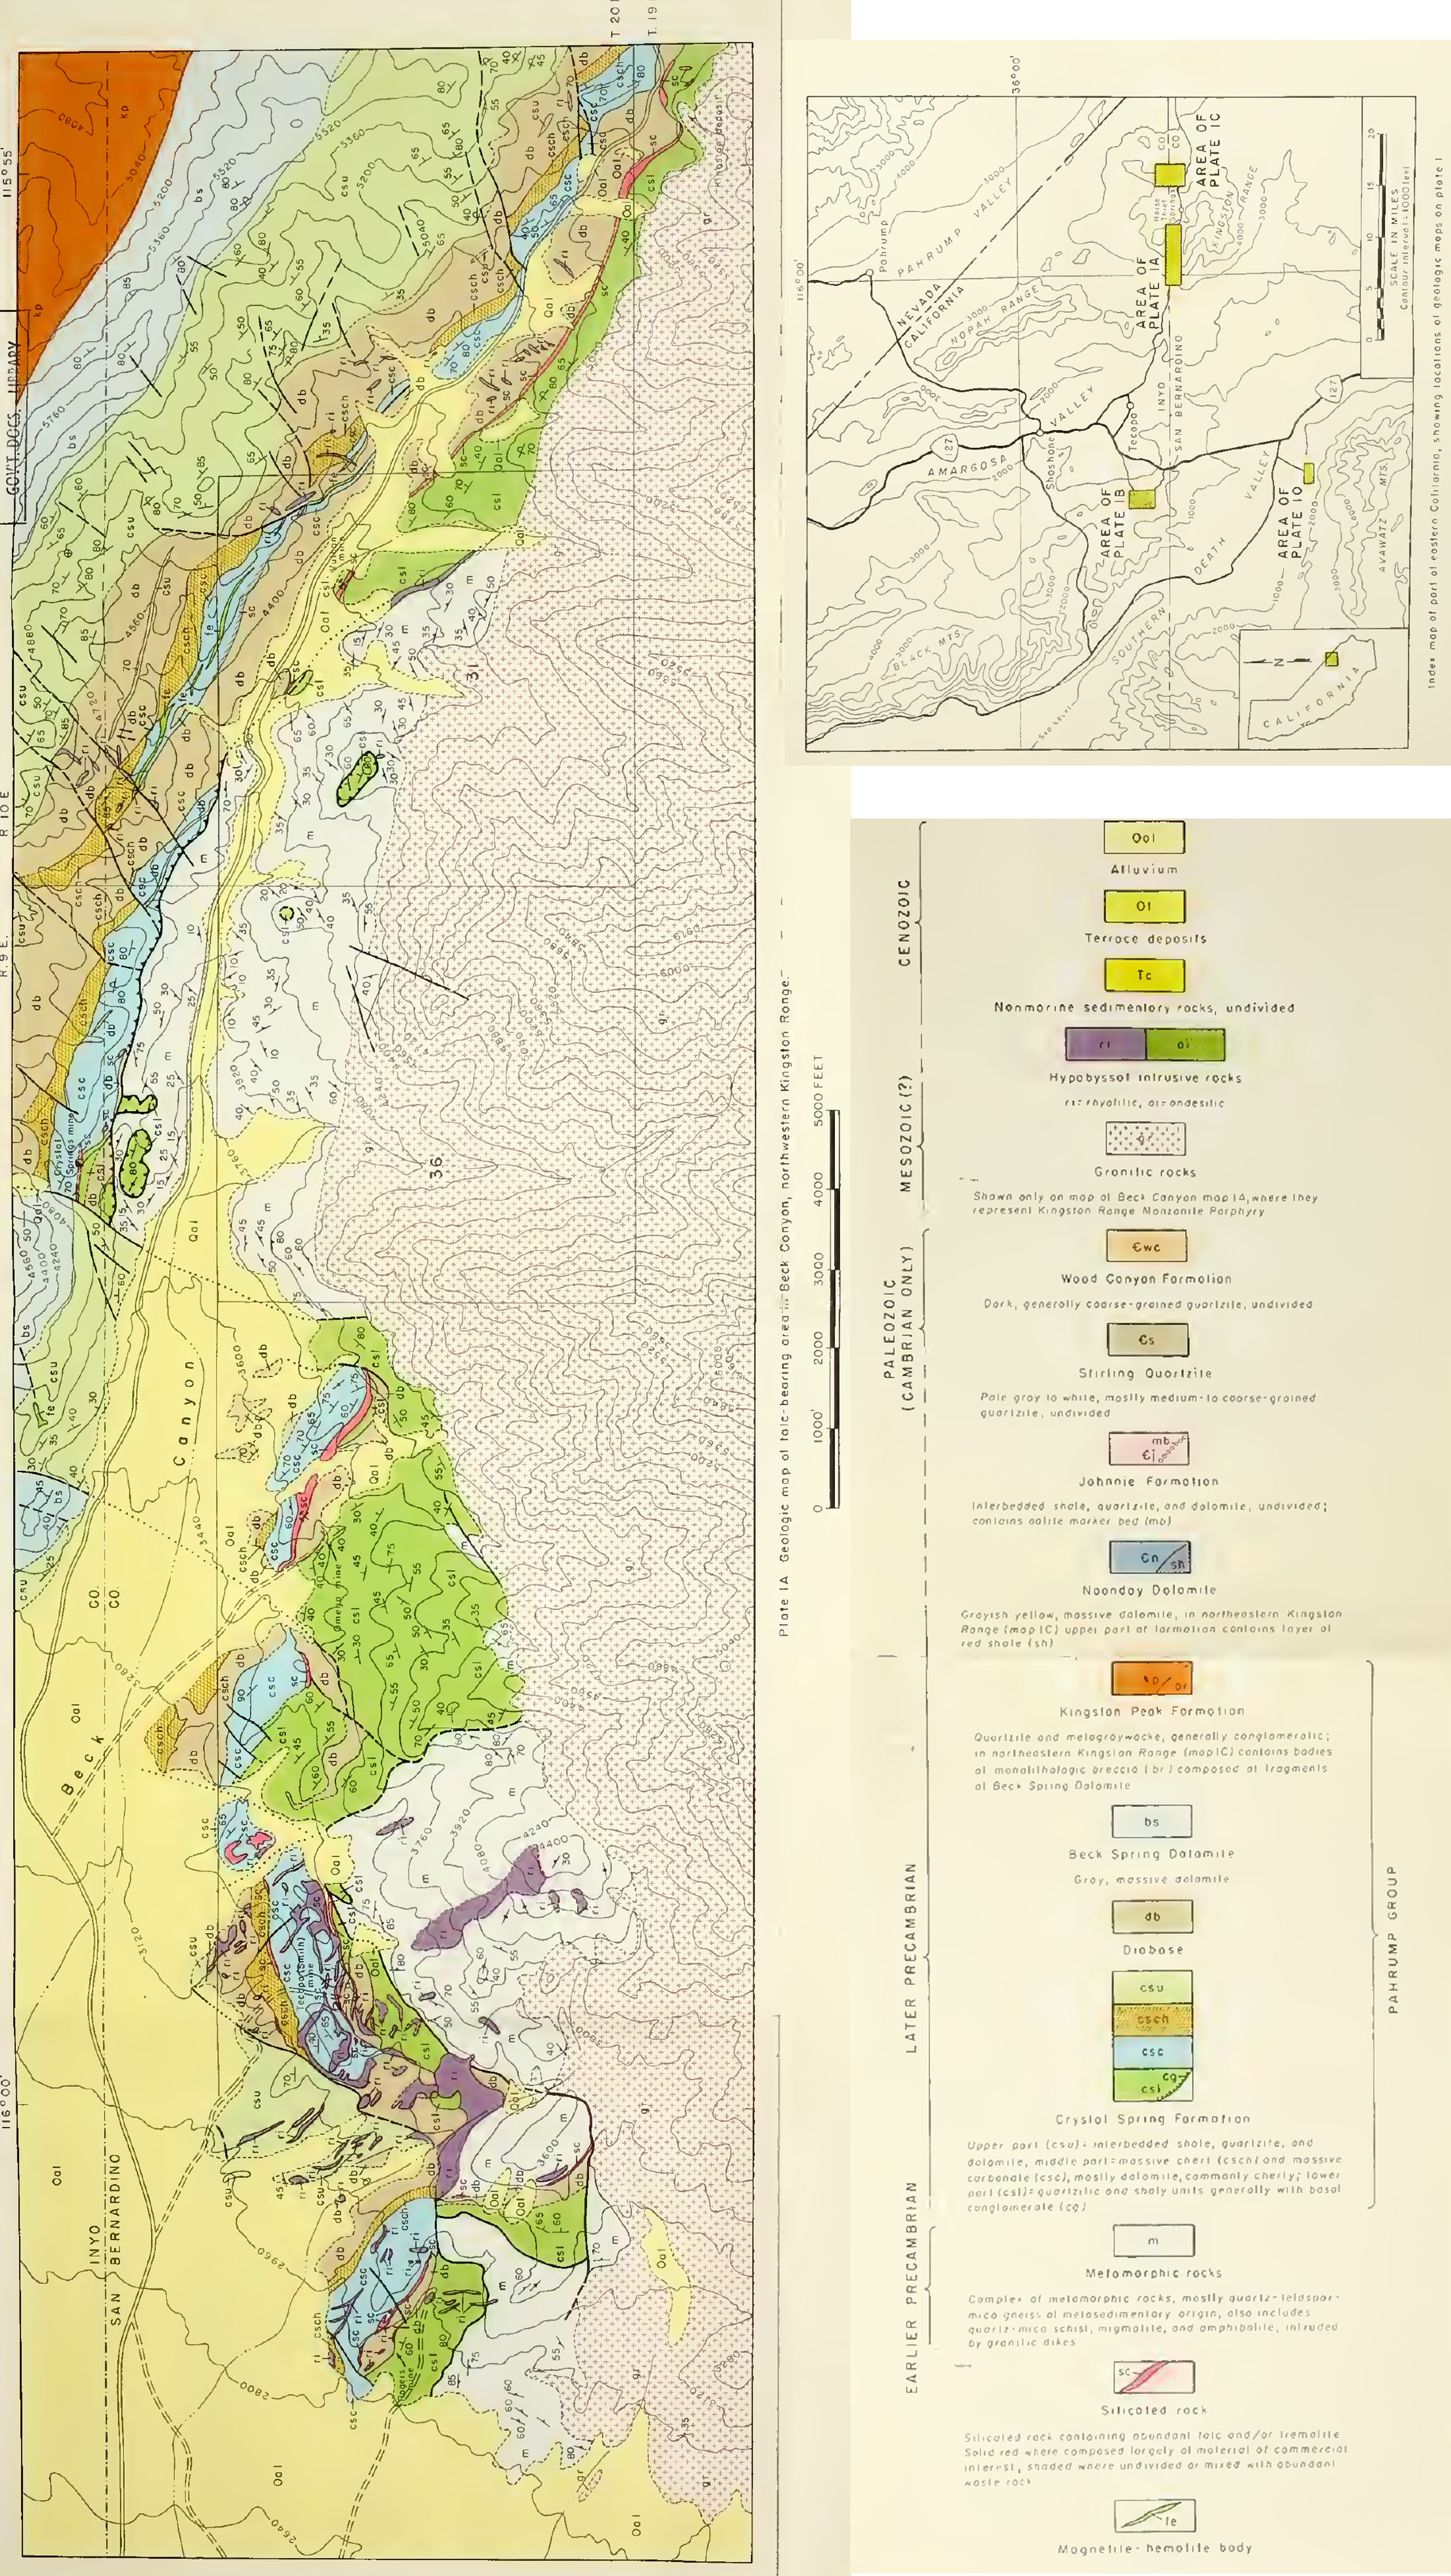
\includegraphics[width=0.8\textwidth]{figures/Wright1968.jpg}
	\caption{caption}
	\label{fig:label}
\end{figure}

\end{document}